\documentclass[letter,12pt]{article}
\usepackage[letterpaper,right=1.25in,left=1.25in,top=1in,bottom=1in]{geometry}
\usepackage{setspace}

\usepackage[utf8]{inputenc}   % allows input of special characters from keyboard (input encoding)
\usepackage[T1]{fontenc}      % what fonts to use when printing characters       (output encoding)
\usepackage{amsmath}          % facilitates writing math formulas and improves the typographical quality of their output
\usepackage{url}              % adds line breaks to long urls
\usepackage[pdftex]{graphicx} % enhanced support for graphics
\usepackage{tikz}             % Easier syntax to draw pgf files (invokes pgf automatically)
\usetikzlibrary{arrows}

\usepackage{mathptmx}           % set font type to Times
\usepackage[scaled=.90]{helvet} % set font type to Times (Helvetica for some special characters)
\usepackage{courier}            % set font type to Times (Courier for other special characters)

\usepackage[longnamesfirst, sort]{natbib}\bibpunct[]{(}{)}{,}{a}{}{;} % handles biblio and references 

\usepackage{rotating}         % sideway tables and figures that take a full page
\usepackage{caption}          % allows multipage figures and tables with same caption (\ContinuedFloat)

\usepackage{dcolumn}          % needed for apsrtable and stargazer tables from R to compile
\usepackage{arydshln}         % dashed lines in tables (hdashline, cdashline{3-4}, 
                              %see http://tex.stackexchange.com/questions/20140/can-a-table-include-a-horizontal-dashed-line)
                              % must be loaded AFTER dcolumn, 
                              %see http://tex.stackexchange.com/questions/12672/which-tabular-packages-do-which-tasks-and-which-packages-conflict


\newcommand{\mc}{\multicolumn}

%% TO ADD NOTES IN TEXT
\usepackage[colorinlistoftodos, textsize=small]{todonotes}
\newcommand{\emm}[1]{\todo[color=blue!30, inline]{\textbf{To do:} #1}}


\begin{document}

\title{Presidential obstruction of the agenda \\in Chile's Congress\thanks{Prepared for presentation at the annual meeting of the American Political Science Association, San Francisco, CA, 9/4/2015. The author is grateful to Jos\'e Antonio Cheibub, Gisela Sin, and participants at the Comparative Politics Workshop of the University of Illinois at Urbana-Champaign for useful comments and critiques; to the Department of Political Science at Washington University in St.\ Louis, where much of this work was done as visiting scholar; and acknowledges financial support from the Asociaci\'on Mexicana de Cultura A.C.\ and CONACYT's Sistema Nacional de Investigadores. The author bears sole responsibility for mistakes and shortcomings in the study.}}
\author{Eric Magar \\ ITAM }
\date{\today}
\maketitle

%\begin{center} \textbf{$\rightarrow$~~Preliminary draft~~$\leftarrow$} \\ (please inquire for new version, \small{\url{emagar@itam.mx}})  \end{center}

\begin{abstract}
\noindent Unlike presidents with mostly (or only) reactive formal powers in the legislative arena, Chile's enjoys formidable proactive ones. Among them is the urgency authority. A bill declared urgent confronts legislators with a short deadline to discuss and vote it. Urgency, research has shown, correlates with the odds of bill passage, and most executive-initiated legislation becomes urgent at some stage. Comparing the Chilean urgency authority to others in the region reveals no penalty for non-compliance, leaving urgency messages as cheap talk unless presidents can persuade legislators that costs indeed exist. I inspect original data of the decision to declare legislation urgent in order to shed light on the disconnect between usage and institutional status. I do not answer what makes the urgency consequential satisfactorily, but the attempt manifests suggestive patterns and raises puzzles worth investigating in future research. 
\end{abstract}

 %Inspection of original data on urgency incidence to investigate the decision to declare or not legislation urgent, an aspect that has received less scholarly attention. Analysis of original data distinguishes messages in the 1998--2014 period that set forth urgency (40\% of 20 thousand), messages that changed the deadline (29\%), and messages to withdraw the bill's urgency (31\%). Isolating bill and session traits that correlate with urgencies sheds light on the president's power to constantly obstruct the legislative agenda and its use in executive-legislative negotiation with separation of power. 

\onehalfspacing

\noindent Part I of the book studied executive-legislative bargaining in presidential democracies with a standard separation of power framework, giving presidents a reactive power only, the authority to veto legislation. Part II gave the president pro-active legislative power, the authority to enact policy unilaterally pending assembly approval. This chapter and the next explore another pro-active presidential power: the ability to interfere with legislative scheduling from the executive branch. 

The paper, which reports work in progress, is a first approach to the study of the urgency authority. A president with urgency authority can remove obstacles preventing floor consideration of legislative proposals. With important variations, five constitutions of the Americas give such authority to the president, Chile's among them. The paper makes three contributions. 

It offers a framework to compare the urgency authority across constitutions. Highlighting the importance of the reversionary policy and reversionary schedule reveals that the Chilean version, unlike those of Brazil, Colombia, and Uruguay, is apparently toothless: urgency summons by the Chilean president are really empty threats. The addition of costly scheduling and costly rejection assumptions offers a way to restore at least part of the institution's might. 

It describes another element of the Chilean variant, the degree of urgency. Urgency degrees define specific deadlines to consider legislation, ranging from less than one to four weeks. Many puzzles arise from observing frequencies of different types of urgency messages in original data. Among the puzzles is an appalling reliance of the urgency authority in four Chilean post-transition Legislatures between 1998 and 2014. The numbers are difficult to reconcile with a view that the urgency authority is inconsequential. *Offer other puzzle. 

And it inspects committee reporting in the lower chamber of Chile's Congress. Unless urgency is raised to speed the scheduling of a committee report for floor consideration, a consequential urgency authority should trigger committee reports in due time. Analysis of weekly reports by the almighty Hacienda committee reveal ripples associated with different degrees of urgency. This is evidence that the authority achieves some of its intended effects despite the lack of teeth.  

%Interfering with the legislative schedule does not end policy differences between the branches per se, and the urgency authority confronts a paradox. Can it convey influence in the legislative arena? Given an urgency, a recalcitrant assembly will simply stop the president's proposal sooner then it would have done. But at least two differences become plainly evident: the timing, whatever had been prioritized by assembly leadership is inevitably pulled down in the schedule by executive fiat; and the action, as legislators will be forced to explicitly bring down the proposal, instead of letting it stand (perhaps indefinitely). Such difference, this chapter aims to show, may put pressure on the legislature and therefore serve as an alternative form of negotiation. This opens up new facets in executive-legislative negotiation. 

The paper proceeds thus. Section 1 briefly reviews empirical studies of the urgency authority, spotting a major obstacle to measure its effects. Section 2 develops a theoretical framework capturing two key institutional elements of the urgency authority: the reversionary policy and reversionary schedule applicable when the assembly misses the urgent deadline. The general perspective reveals a flaw in the Chilean variant, compared to the Brazilian, Colombian, and Uruguayan. Including costs associated with scarce time and presidents who can persuade offers a way to restore some of the Chilean institutions bite. Section 3 looks at the details of Chile's urgency authority. The particular perspective identifies urgency degrees, and speculates about this element's potential to make the urgency authority consequential. Section 4 introduces an original dataset of bill histories and urgency messages in Chile in the 1998--2014 period. Many puzzles arise from the descriptive statistics on bill initiation, bill passage, and urgency usage. One is the disconnect between a possibly inconsequential institution and the remarkable frequency of its use. Section 5 inspects committee reporting following different types of urgency messages. Analysis shows that, far from inconsequential, the urgency authority indeed lets Chilean presidents determine legislative scheduling. Section 6 offers closing remarks. 


\section{The received wisdom}

\begin{center}
\singlespacing
[U]rgency powers... can have dramatic effects on executive-legislative \\ 
relations, legislative organization, and the policy process more generally\\ 
---\citet[][:438]{morgenstern.2002b}
\end{center}
\onehalfspacing

%\citeauthor{carey.shugart.1998a}'s \citeyearpar{carey.shugart.1998a} monograph on executive unilateral powers does not discuss it. \citeauthor{londregan.2000a}'s \citeyearpar{londregan.2000a} study of legislative institutions in the Chilean Senate does not include the urgency authority in the index. 

\noindent The urgency authority has received relatively little scholarly attention. While not discussing it directly, \citeauthor{carey.shugart.1998a}'s \citeyearpar{carey.shugart.1998a} elaboration of the delegation of unilateral authority to the executive offers clues about the logic behind the institution. Informational/valence asymmetries between Latin American executive and legislative branches \citep{londregan.2000a} create incentives for delegation. Delays to reach agreement may also diminish the value of policy \citep{baron.ferejohn.1989}, so rather than delegate proposal power within the chamber, legislators may prefer to see the president set the agenda. 

%\citet{siavelis.2002} is the first study to cover the urgency authority. He hypothesized urgencies' game-changer potential. His study of Chilean executive-legislative covers the first post-transition presidency revealed just how very frequently urgency messages were issued: slightly more than one-third of proposals in Congress received some form of urgency, and about 9 out of 10 of urgent bills were executive-initiated. Guided by semantics, analysis sought to discover if urgent bills, in fact, circulated the steps of the legislative process faster than the rest, and whether urgency status also increased the likelihood of bill passage. The study found mixed evidence. Among executive bills, consideration of urgent ones had somewhat shorter duration than the rest (medians of 134 and 160 days, respectively), but no palpable difference in success rates is appreciated (64 and 63 percent, respectively). 

\citet{siavelis.2002} is the first study to cover the urgency authority. Like Morgenstern's quote, he hypothesized the urgency power's game-changer potential. His study of Chilean executive-legislative in the first post-transition presidency revealed the amazing frequency with which urgency messages were issued by President Aylwin: slightly more than one-third of proposals in Congress received some form of urgency, and about 9 out of 10 of urgent bills were executive-initiated. This poses the chapter's first major puzzle. \citeauthor{berrios.gamboa.fiscChile.2006}'s \citeyearpar{berrios.gamboa.fiscChile.2006} study of budgetary congressional oversight of the executive warns against overstating the urgency authority's importance, as non-compliance does not have approval of the proposal as a consequence---the next section develops this argument. Why would presidents resort so frequently to an authority that is potentially inconsequential?

Guided by semantics, Siavelis also sought to discover if urgent bills, in fact, circulated the steps of the legislative process faster than the rest, and whether urgency status increased the likelihood of bill passage. The study found mixed evidence at best. Among executive bills, consideration of urgent ones had somewhat shorter duration than the rest (medians of 134 and 160 days, respectively), but no palpable difference in success rates is appreciated (64 and 63 percent, respectively). The negative finding is partly attributable a failure to control for urgency degrees (discussed in section 3) in the analysis. \citeauthor{aleman.navia.UrgChi.2009}'s \citeyearpar{aleman.navia.UrgChi.2009} systematic study of executive success in Congress in three post-transition presidencies explicitly controlled for urgency degree, finding some of the evidence sought by Siavelis. Controlling for bill characteristics (such as key policy domains, the chamber where the bill originated, the government seat margin, and presidential approval) and clustering errors by legislative year (to capture heterogeneity of grandly changing presidential agenda sizes), urgency degrees had quite different effects in passage. And they found that higher degrees are significantly associated with increased probability of executive bill passage, but the lower (which is also much more common, as will be seen) made no statistical difference. 

% longer review of aleman and navia
%\citeauthor{aleman.navia.UrgChi.2009}'s \citeyearpar{aleman.navia.UrgChi.2009} systematic study of executive success in Congress in three post-transition presidencies also inspects Chile's urgency authority. Among controls, their equation includes urgency authority usage in the right side. The unit is the individual bill, and the size of the executive agenda varies substantially over the years. Variation is quantitative  (Congress received about 150 presidential bills in each of the first 6 years after 1990, a numbrer that dropped to about 70 in the next 6 years, then climbed to about 100 in the final 4 years of their series) and qualitative, presidents manifesting different propensities to aim at constitutional reform. Of direct relevance are the findings on urgencies. Controlling for key policy domains, chamber of origin, seat margins, and presidential approval, and clustering errors by legislative year, different prioritization reveal quite different effects in passage. `Act now' and `2-week' notices significantly increased the probability of bill passage, but not `4-week' notices. 

The negative finding may also be attributable to selection bias: the set of bills receiveing urgent status is not random. Presidents, behaving strategically, are likely to target for urgency proposals that are markedly different from the rest in important ways. The problem of endogeneity that arises poses an obstacle to measure urgency authority effects. Separating effects requires more subtle methods than used up to now. Like the Siavelis and Alem\'an-Navia studies, this chapter recognizes the problem but does not confront it methodologically. Until a better identification design is proposed, findings must be taken with a grain of salt. Yet the hope is that urgency correlations with different steps and outcomes of the Chilean legislative process offered here will help pave the way to a solution. 

%If presidents, behaving strategically, were to target for urgency proposals that are markedly different from the rest in important ways, a problem of endogeneity arises. Classify proposals based on how difficult passage is expected: easy, hard, and impossible. If left on their own, the easy proposals would be approved faster, the hard slower, the impossible never. A strategic president should concentrate the urgency authority in the hard group, leaving easy proposals mostly on their own, while abandoning the hopeless group of impossible proposals, that will not be observed. As a consequence, comparing

%The relevant quantity of interest is whether the use of the urgency authority affects bill passage (success, speed, amendments, and so forth) compared to the same bill with no urgency attached. The fundamental problem of causal inference is immediately evident. The executive presumably targets bills for urgency strategically, so that the selection mechanism cannot be assumed random. If, for example, more complex and divisive legislation takes longer, is likelier to fail and likelier to be tagged urgent, separating effects requires more subtle methods than used up to now.


\section{Costly scheduling and inaction}

Five constitutions of the Americas give executives the power to interfere, to some degree, with the assembly's voting schedule. The urgency authority varies considerably \citep[][:437]{morgenstern.2002b}. In Brazil, the assembly must act on a bill deemed urgent withing 45 days, or else it takes precedence over all other legislative business. The president can declare any executive-initiated bill urgent at any time. And, since 2001, all executive unilateral policy (\emph{medidas provis\'orias}) become urgent bills upon publication. In Colombia, an urgent bill goes to the top of the voting schedule immediately. In Uruguay and Chile, legislators must act withing a pre-specified, short period; failure to do so converts the urgent bill into law in Uruguay---although three-fifths of any chamber's membership can remove the project's urgent status. As said, in Chile the consequences of inaction are indetermined. And in Mexico since 2012, the president can declare up to four bills urgent every year, which must scheduled for floor consideration within 30 days.\footnote{Constitutional articles where this authority is established: Brazil 62 and 64; Chile 74; Colombia xx; Mexico 71; and Uruguay 168.7.}

%\emm{How does this compare with extra-ordinary sessions? Some presidents can summon legislators to a special session to discuss, exclusively, a specific bill defined ex-ante. Limits? If few, might resemble urgency authority... Check}

\begin{figure}
  \centering
    \tikzstyle{mid}=[circle,draw]
    \begin{tikzpicture}
      \node[mid] at (2,-.5) (e) {\emph{E}}; 
      \node[mid] at (4,1) (l) {\emph{L}}; 
      \node[right] at (4,-2) (ee) {$x_0+o$}; 
      \node[right] at (6, 2.5) (le1) {$x_1$};  
      \node[right] at (6, 1) (le3) {$x_0-c$}; 
      \node[right] at (6,-.5) (le2) {$r+o-k$}; 
      \path[-]  (e) edge node [above, sloped] {\footnotesize{propose}} (l);
      \path[]   (e) edge node [below, sloped] {\footnotesize{$x_1$}}   (l); 
      \path[-o] (e) edge node [below, sloped] {\footnotesize{not}}     (ee) 
                 (l) edge node [above, sloped] {\footnotesize{accept}} (le1) 
                 (l) edge node [below, sloped] {\footnotesize{ignore}} (le2);
      \path[-o] (l) edge node [above, sloped] {\footnotesize{reject}} (le3);
    \end{tikzpicture}  \\
 \footnotesize{
 \begin{tabular}{lrrr}
  Case                       & $r$   & $c$   & $k$      \\ \hline
  Chile                      & $x_0$ & 0     & $>0$     \\
  Brazil (urgency), Colombia & $x_0$ & 0     & $> o$    \\
  Brazil (MP)                & $x_0$ & $>0$  & $> o$    \\
  Brazil (MP up to 2001)     & $x_1$ & $>0$  & 0        \\
  Mexico (4 bills yearly)    & $x_0$ & 0     & ?        \\
  Uruguay                    & $x_1$ & 0     & 0        \\
  \end{tabular}
  }
\caption{Urgency authority and costly scheduling and rejections}\label{f:costly}
\end{figure}

Figure \ref{f:costly} offers a framework, similar to that used throughout the book, to compare different urgency authorities. Key in the stylization is that the rejection of undesirable executive proposals as entailing costs for the assembly. The framework reveals similarities and differences between urgency authorities, and their consequences for executive-legislative bargaining. The frame is set as a two-player game between the executive and the pivotal legislator. The executive starts by proposing urgent policy $x_1$, or ending the game with the status quo $x_0$ in place. Terminal nodes in the game tree indicate the policy outcome and associated costs (all elaborated below). Costs are all borne by the legislator, whose payoff is the value of the policy outcome indicated and the value of the costs: in the case of the bottom terminal node, for instance, this would be $u_l(x_0)+o$ (where $u_l$ is spatial utility). 

Given scarce committee and plenary time, scheduling anything for consideration entails an opportunity cost $o$. Conceptually, $o$ is the value of the best alternative policy that the legislator might adopt if scheduled instead of proposal $x_1$. With an institution that no two (or more) proposals are scheduled simultaneously, considering $x_1$ inevitably postpones the consideration of the best alternative---indefinitely, perhaps, since the agreement to schedule it next may break down. So, whenever the executive makes no proposal in the framework, value $o$ can be realized by the legislator in the bottom terminal node (he is free to schedule the alternative), adding up to the policy payoff. 

If called to play, the legislator faces three actions to choose from, all leading to terminal nodes. For ease of exposition, costs other than $o$ are initially set to zero ($c = k = 0$), cancelling out of the description. The restriction is relaxed afterwards. The legislator can accept the proposal, replacing the status quo with policy at $x_1$. This choice entails an opportunity cost, and therefore $o$ cannot be realized. The legislator could alternatively retain the status quo by rejecting the proposal, a choice also putting $o$ beyond reach due to the need to schedule the bill for rejection. And the legislator could opt to ignore the proposal, policy reverting to a pre-defined reversion outcome $r$. Unlike the other alternatives, ignoring frees legislative time to schedule something else, and $o$ adds to the value of the outcome. 

% Mex: exec-init actually rejected (diputados Weldon)
% 58 none
% 59 4 down (3 negative reports, 1 voted)
% 60 4 down (2 negative reports, 2 voted) (both voted and 1 report were carry-overs from Fox's)
% 61 2 down (1 negative report, 1 voted) (report was carry-over from Fox's) (preclusión adopted here: after 45-90 days with no report, Mesa can archivar proposals... a bunch were precluidas en bloc)
%
% Mex: exec-init passed (diputados Weldon, includes minutas)
% 2000-01 21
% 2001-02 30
% 2002-03 29
% 2003-04 16
% 2004-05 32
% 2005-06 23
% 2006-07 15
%
% Mex: ex-init (diputados infosil, excludes minutas and carryovers)
% 58: 63 in, 55 approved
% 59: 49 in, 31 approved
% 60: 42 in, 38 approved
% 61: 32 in, 26 approved
%
% Synthesis of Weldon/Infosil data
% 58:  63 in,  55 approved, 0 rejected,  8 ignored
% 59:  49 in,  31 approved, 4 rejected, 14 ignored
% 60:  42 in,  38 approved, 1 rejected,  3 ignored 
% 61:  32 in,  26 approved, 1 rejected,  5 ignored
% all:186 in, 150 approved, 6 rejected, 30 ignored
%
%          period       exec-init   rechazadas  retiradas  aprobadas pendientes
% Chile    1998-2014      1469                113            1075       281
% Br       1995-2010      1650          73         109       1100       367
% Urug     1995-2005      1050                                709
% Urug     1985-1990       416                                269
% Urug     1985-2000      1456                                965

\begin{table}
\centering
\begin{tabular}{lcrrrrr}
Case   & Period     & Withdrawn & Rejected & Pending & Total & (N) \\ \hline
Brazil & 1995--2010 &  13       &   20     &   67    &  100  & (549) \\
Chile  & 1998--2014 & \mc{2}{c}{29}        &   71    &  100  & (394) \\
Mexico & 2000--2012 &   0       &   17     &   83    &  100  &  (36) \\
\end{tabular}
\caption{How executive bills failed in three cases. Sources: Mexican executive bill approval is from \protect\url{http://sil.gobernacion.gob.mx}, rejections kindly shared by Jeff Weldon. Gobernaci\'on reports carry-over bills from previous Legislaturas in a residual category, and some bills ignored by the current Legislatura were in fact considered by subsequent ones in the period. Of these, 4 more were actually rejected (3 by negative report, 1 by floor vote).}\label{t:exBillFail}
\end{table}

Reversionary policy $r$ varies across constitutions, alternating between the status quo ante and the executive's proposal ($r\in\{x_0,x_1\}$). The Uruguayan reverts policy to executive proposals declared urgent but not scheduled for a vote ($r=x_1$); the rest revert to the status quo ante ($r=x_0$). The Brazilian was like the Uruguayan in cases of urgency by \emph{medida provis\'oria} up to 2001, when the constitution was amended.\footnote{\emph{Medidas provis\'orias} expire 60 days after publication. Before the reform, a Supreme Court ruling legalized the option of re-issuing MPs that had not been discussed and voted in Congress upon expiration, leading to the instituion described in the text ($r=x_1$). The reform adopted 9/11/2001 limits to one re-issue, with urgency kicking in case of congressional inaction. See \citet{figueiredo.etal.1996}.} Absent costs other than $o$, ignoring dominates rejecting undesirable proposals, foregoing opportunity costs (this claim ignores the possibility of $o<0$). This jibes with evidence of assemblies brushing aside undesired executive proposals by inaction rather than actual rejection. (In three cases reported in table \ref{t:exBillFail}, two-thirds or more of failed executive proposals remained pending in Congress (in Brazil and Chile) or the lower chamber (in Mexico). The rate is highest in Mexico, which has the most limited urgency authority, and lowest in Brazil, which has the least limited.) The alternative reversion policy $r=x_1$ brings a drastic change in executive-legislative relations, as congressional inaction becomes a way of adopting presidential policy more cheaply.\footnote{The game tree ignores the possibility in the Uruguayan constitution of overriding the urgency authority. Three-fifths of the membership of either chamber of Parliament can vote to strip the proposal of urgent status. A successful override returns $r=x_0$.} 

Relaxing the nil costs restriction brings further depth into the comparative framework. Cost $c>0$ lowers the value of the status quo by rejection for the legislator. This cost is associated with unilateralism per se, independent of the urgency authority, and therefore is applicable to the Brazilian case only (where both institutions are compounded since 2001). \emph{Medidas provis\'orias} are presidential decrees with immediate force of law, and unlike statutory proposals, they turn potential into actual winners and losers before the assembly votes on them. At the statutory proposal stage, there is an expectation that a group might receive a flow of benefits if all goes according to plan. A fair amount of uncertainty surrounds all, both about the likelihood that policy will in fact materialize and about the size and scope of benefits associated with the details of the policy that eventually passes. Once adopted, however, this uncertainty vanishes. When policy is adopted unilaterally, winners and losers are clearly identified before the measure is discussed and voted, changing the obstacles that the assembly may face. Rescinding the decree will imply surmounting an identifiable opposition that could organize more cheaply than the diffuse kind \citep{olson.1965} anticipating policy by statute. This translates into cost $c>0$.  

Cost $k>0$ mitigates, or even cancels, the value of the opportunity cost realized by ignoring the president's proposal. It is associated with higher salience achieved by tagging a proposal ``urgent''. By signaling presidential priority, coupled with a clever communication strategy, the urgency authority may contribute to place an issue in the public agenda, increase media attention, and nurture public debate. An undesired proposal that could have easily been dusted under the carpet in normal circumstances will, as a consequence of increased salience, be harder to duck---adding a cost. Cost $k$ is magnified when the institution brings an urgent but unconsidered proposal to the top of the assembly's Day's Order. At this point, continuing to ignore proposal $x_1$ starts to subtract value of $o$ once for every extra subsequent session that the executive proposal continues to not be considered---i.e., $k>o$. 

Cost $k>0$ mitigates, or even cancels, the value of the opportunity cost realized by ignoring the president's proposal. It relates to policy salience and what \citet{neustadt.1990} called the president's power to persuade. Raising urgency conveys a sense of the issue's importance and of imperative immediate attention. By signaling presidential priority, coupled with a clever communication strategy, the urgency authority may contribute to place issues in the public agenda, increase media attention, and nurture public debate. An undesired proposal that could have easily been dusted under the carpet in normal circumstances will, as a consequence of increased salience, be harder to duck---adding a cost. Cost $k$ is magnified when the institution brings an urgent but unconsidered proposal to the top of the assembly's Day's Order, as in Colombia and Brazil. At this point, continuing to ignore proposal $x_1$ subtracts value $o$ once for every additional session until the proposal is considered---i.e., $k>o$. 

The table accompanying Figure \ref{f:costly}'s game tree summarizes costs associated with rejection and ignoring urgent proposals in the five constitutions. Cost $c>0$ is present in Brazil's unilateralism only, and $r=x_1 \rightarrow k=0$ (ignoring urgency in such case is a tacit acceptance of salient policy). In Mexico, the consequences of inaction remain indeterminate---a future Supreme Court ruling or legislation might fill the blank. 

The next chapter analizes the Brazilian case. Analysis of the Chilean variant, using Uruguay as a baseline, is done next.

\section{Degrees of urgency in Chile}

Formal executive authority to interfere in the Congressional agenda in Chile has constitutional status. The constitution (art.\ 74) stipulates that the president can urge action on any bill (not just executive proposals) at any stage of the legislative process. The chamber receiving the urgency message is compelled to act on the bill (``discuss and vote it'') before a deadline. Since inter-cameral differences are dealt with in conference in the Chilean bicameralism (\emph{comisión mixta}, const.\ arts.\ 68--70), an urgency message at this stage compells Congress (i.e., the conference and then each chamber) to act before the deadline. 

The Congressional Organic Law (arts.\ 26 and 27) defines the breadth of the interference, giving the president a choice of sending a `four week notice' (\emph{urgencia simple}), a `two week notice' (\emph{urgencia suma}), or an `act now' (\emph{discusión inmediata}) message. The Organic Law was amended in July 2010, somewhat relaxing the deadlines for the `act-now' and `two-week' urgencies, stretching from 10 to 15 and from 3 to 6 days, respectively. `Four-week' urgencies stayed put, at 30 days. Issuing maximum urgency in the right circumstances---an act-now message attached to a bill in conference before 2010---gave each instance just one day to act: one for the conference to report a compromise bill, and one for each chamber to sequentially consider and push the bill to the floor for a vote (congressional practice is well summarized by the library of Congress at \url{http://www.bcn.cl/ecivica/formacion/}.) The president may remove the urgency at will, with immediate effects. With the exception of bills in conference, urgency targets business in the chamber receiving the message only, and expires at the end of the ordinary period on March 10th every year. 

The constitutional bases of the urgency authority, it must be noted, are minimal. In fact, the constitution defines low-degree urgency only (when urgency is raised, Congress must act before 30 days have passed). Higher degrees are defined in the organic law only. This could make higher-degree urgency vulnerable to congressional majorities, who might be inclined to relax the degrees of urgency available to the president if that were in their interest---as, in fact, was done in 2010. But the constitution (art.~66) also raises the requirement organic law passage and amendment, whose approval requires the vote of four-sevenths ($\approx 57$ percent) of each chamber's membership. While less strict than that the two-thirds membership needed for constitutional reform, the super-majority is considerable nonetheless. 

Vagueness surrounds key aspects of Chile's urgency authority. When a 30-day limit is set, for instance, no indication is given of whether those are calendar, business, or session days. I treat the messages in weeks rather than days given imprecision (and, when coding deadlines in the empirical sections below, arbitrarily rely on business days). More important, unlike the institution in Brazil, Colombia, and Uruguay, no formal course of action (or reversionary schedule) is defined in case of failure by the chamber to act on the bill upon the deadline's expiration. And no hint of rulings by the Constitutional Tribunal filling in the institutional void could be found. By default, I interpret indeterminacy as reversion to the status quo ante ($r=x_0$) with no effect on the voting schedule.\footnote{How is the Day's Order (\emph{tabla}) prepared in each chamber? Investigating scheduling in each chamber should illuminate the question. Both Constitution and Organic Law remain silent about this.} 

In the absence of a formal penalty for inaction---like Uruguayan reversion to $x_1$ absent an urgency-removing supermajority; or placing Brazilian legislative business on hold until the urgency is heeded---only cost $k$ remains to effect a possible change in the Chilean assembly's actions. In other words, whenever $k=0$, ignoring a proposal dominates rejecting it (strongly so, unless $o+c=0$). This observation dovetails with previous characterizations of the Chilean urgency authority. \citet{berrios.gamboa.fiscChile.2006} advance the notion that, in spite of reversion $r=x_0$, the assembly may indeed face political costs of ignoring urgency messages on salient proposals. 

The president's qualification of the urgency offers some elements to investigate this last point. In line with \citet{aleman.navia.UrgChi.2009}, I relate cost $k$'s size to the urgency degree---higher degrees let the president make louder statements to raise issue salience. So, all else equal, a `two week' notice has a larger $k$ (or, at least, never lower) than a `four week', and an `act now' message has a larger $k$ (or, at least, never lower) than either other. Urgency type frequency, in fact, reveals a tendency to rely less often on more urgent messages (descriptive data is presented in the next section). `Act now' notices were roughly 3 to 5 times less frequent than `two week' ones in a recent 16-year period. The frequency differential between `two' and `four week' notices is less sharp, but a tendency is distinguishable. 

Isolating the Chilean version of the game in Figure \ref{f:costly}, and contrasting it to the Uruguayan, reveals how the size of $k$ relative to $o$ and the reversion point determine who is advantaged by the urgency authority. Figure \ref{f:chiUruEql} does this. The Uruguayan institution in the right panel necessitates an urgent presidential proposal, or else the $r=x_1$ reversion does not kick in, and the game becomes identical to Chile's. The Chilean institution, in the left panel, allows varying degrees of urgency, from none to `act now'. As urgency goes up, so does the size of cost $k$, monotonically. Proceeding backwards in the Chilean setting, the legislator compares relative values of three outcomes: $x_1$, $x_0$, and $x_0-k+o$. Unlike the first outcome, the others are defined exogenously, and therefore serve to set a baseline for the legislator's optimal reaction to the president's proposal. Giving players specific preferences relative to the status quo aides in seeing the bargaining logic and institutional effects. An interesting example is $x_0 < l < p$, leaving room for inter-branch compromise in policy, is analyzed graphically below the game tree in the figure. (I do not derive the full equilibrium, which is in line with the model in chapter 2). 

\begin{figure}
  \centering
\begin{tabular}{c|c}
   Chile & Uruguay \\
    \tikzstyle{mid}=[circle,draw]
    \begin{tikzpicture}[scale=0.7]
      \node[mid] at (2,-.5) (e) {\emph{E}}; 
      \node[mid] at (4,1) (l) {\emph{L}}; 
      \node[right] at (4,-2) (ee) {$x_0+o$}; 
      \node[right] at (6, 2.5) (le1) {$x_1$};  
      \node[right] at (6, 1) (le3) {$x_0$}; 
      \node[right] at (6,-.5) (le2) {$x_0-k+o$}; 
      \path[-]  (e) edge node [above, sloped] {\footnotesize{prop.}} (l);
      %\path[]   (e) edge node [below, sloped] {\footnotesize{$x_1$}}   (l); 
      \path[-o] (e) edge node [below, sloped] {\footnotesize{not}}     (ee) 
                 (l) edge node [above, sloped] {\footnotesize{acc.}} (le1) 
                 (l) edge node [below, sloped] {\footnotesize{ign.}} (le2);
      \path[-o] (l) edge node [above, sloped] {\footnotesize{rej.}} (le3);
    \end{tikzpicture}
         &
    \tikzstyle{mid}=[circle,draw]
    \begin{tikzpicture}[scale=0.7]
      \node[mid] at (2,-.5) (e) {\emph{E}}; 
      \node[mid] at (4,1) (l) {\emph{L}}; 
      \node[right] at (4,-2) (ee) {$x_0+o$}; 
      \node[right] at (6, 2.5) (le1) {$x_1$};  
      \node[right] at (6, 1) (le3) {$x_0$}; 
      \node[right] at (6,-.5) (le2) {$x_1+o$}; 
      \path[-]  (e) edge node [above, sloped] {\footnotesize{prop.}} (l);
      %\path[]   (e) edge node [below, sloped] {\footnotesize{$x_1$}}   (l); 
      \path[-o] (e) edge node [below, sloped] {\footnotesize{not}}     (ee) 
                 (l) edge node [above, sloped] {\footnotesize{acc.}} (le1) 
                 (l) edge node [below, sloped] {\footnotesize{ign.}} (le2);
      \path[-o] (l) edge node [above, sloped] {\footnotesize{rej.}} (le3);
    \end{tikzpicture}
         \\
  \mc{1}{l|}{Case 1: $k<o$} & \mc{1}{l}{Case 3: $k \equiv 0$} \\
          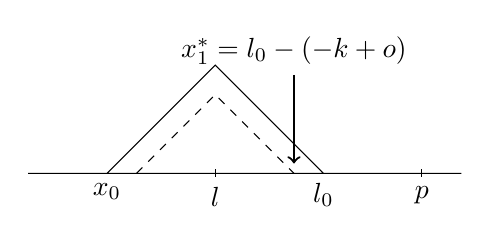
\begin{tikzpicture}[scale=0.5]
          \draw (0,0) -- (11,0) 
          (2,0) node[below] {$x_0$} -- (4.75,2.75) -- (7.5,0) node[below] {$l_0$}; 
          \draw[dashed] 
          (2.75,0) -- (4.75,2) -- (6.75,0); 
          \draw (4.75,0.1) -- (4.75,-0.1) node[below] {$l$}
                (10,0.1) -- (10,-0.1) node[below] {$p$};
          % \draw[->] 
          %       (7,-1) node[below] {$(l_0+o)$} -- (7,-0.25);
          \draw[->, thick] 
                (6.75,2.5) node[above] {\textbf{$x_1^*=l_0-(-k+o)$}} -- (6.75,0.25);
        \end{tikzpicture}
         &
        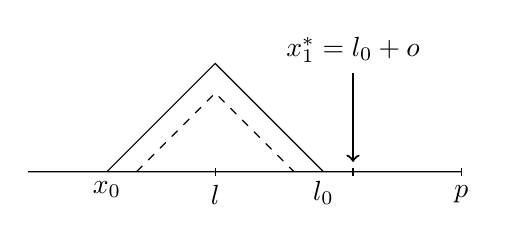
\begin{tikzpicture}[scale=0.5]
          \draw (0,0) -- (11,0) 
          (2,0) node[below] {$x_0$} -- (4.75,2.75) -- (7.5,0) node[below] {$l_0$}; 
          \draw[dashed] 
          (2.75,0) -- (4.75,2) -- (6.75,0); 
          \draw (4.75,0.1) -- (4.75,-0.1) node[below] {$l$}
                (11,0.1) -- (11,-0.1) node[below] {$p$}
                (8.25,0.1) -- (8.25,-0.1) ;
          % \draw[->] 
          %       (8,-1) node[below] {$(l_0-o)$} -- (8,-0.25);
          \draw[->, thick] 
                (8.25,2.5) node[above] {\textbf{$x_1^*=l_0+o$}} -- (8.25,0.25);
        \end{tikzpicture}
         \\
  \mc{1}{l|}{Case 2: $k \geq o$} &  \\
        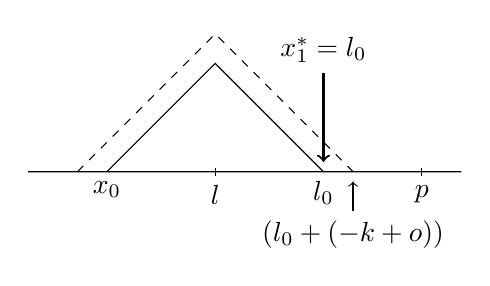
\begin{tikzpicture}[scale=0.5]
          \draw (0,0) -- (11,0) 
          (2,0) node[below] {$x_0$} -- (4.75,2.75) -- (7.5,0) node[below] {$l_0$}; 
          \draw[dashed] 
          (1.25,0) -- (4.75,3.5) -- (8.25,0); 
          \draw (4.75,0.1) -- (4.75,-0.1) node[below] {$l$}
                (10,0.1) -- (10,-0.1) node[below] {$p$};
          \draw[->] 
                (8.25,-1) node[below] {$(l_0+(-k+o))$} -- (8.25,-0.25);
          \draw[->, thick] 
                (7.5,2.5) node[above] {\textbf{$x_1^*=l_0$}} -- (7.5,0.25);
        \end{tikzpicture}
         &
         \\
       \end{tabular}
\caption{Equilibrium costly-scheduling proposals in three cases}\label{f:chiUruEql}
\end{figure}

The Chilean legislator's optimal choice depends, when holding the president's proposal constant, on the $-k+o$ term. Using the standard notation and spatial assumption used throughout the book, $l_0$ in the figure is that alternative leaving the legislator indifferent vis-\`a-vis the status quo (before netting any other costs). While ignoring leaves the status quo intact, it also adds $-k+o$ to the legislator's utility, and the net value of ignoring must be read through the dashed indifference sets. Whenever the opportunity cost more than counters the ignoring cost (i.e., $k<o \leftrightarrow -k+o>0$, as in the figure's case 1), ignoring gives a bonus and therefore dominates rejecting. So, if the president calibrates a proposal at $x_1 = l_0$---which, in the standard game, prompts acceptance---the legislator is better off ignoring it (thus receiving $x_0$ at the dashed value, which is closer to his ideal point $l$ than the proposal's value). The president must therefore make further concessions in order to get the proposal accepted (a proposal at $x_1=l_0-(-k+o)$ leaves the legislator indifferent). 

When $k\geq o$ (as in case 2), the dashed line falls beyond the legislator's costless indifference set, and rejecting dominates ignoring. In such case, a proposal at $x_1=l_0$ is accepted.\footnote{This claim assumes that, when indifferent between accepting and rejecting, the legislator chooses the former. Locating the proposal at $x_1=l_0-\epsilon$ ($\epsilon>0$ tiny), as in chapter 2, achieves the same without this assumption, but is less economical in notation.} And in case 3, where only cost $o$ intervenes (and is assumed positive), ignoring dominates accepting, leaving the executive room to extract welfare from the legislator. Ignoring a proposal at $x_1=l_0$, valued with the dashed line (which, given $o>0$, is contained by the costless indifference set), dominates both accepting and rejecting. With that in mind, an alternative proposal at $x_1=l_0+o$, leaving the legislator indifferent, will still be ignored but with fewer executive concessions. 

In sum, unlike the $r=x_1$ institution, urgency authority with costly time and $r=x_0$ never operates in favor of the executive, as the legislator may gain further influence in policy bargaining. Executive-legislative influence is re-balanced in Chilean-type urgency when cost $k$ is large enough to compensate the legislator's opportunity cost. That could be achieved by lowering the size or $o$, or by raising the size of $k$. Proposing relevant policy (i.e., labeling ``urgent'' an objectively urgent issue) drops the size of $o$, suggesting urgency messages should be rare. The evidence contradicts this expectation. And raising the urgency degree brings the size of $k$ up, begging the question of why should presidents ever issue low-urgency messages.  

Using the authority on objectively ``urgent'' issues drops the size of $o$, suggesting urgency messages should be rare. And raising the urgency degree brings the size of $k$ up, begging the question of why should presidents ever issue low-urgency messages. The evidence in the next section contradicts both expectations, raising additional puzzles. 

%This leads to another puzzle: Why are `four-week' messages so numerous?\footnote{Quoting a former legal chief of staff at the Presidency, \citeauthor{berrios.gamboa.fiscChile.2006} describe `four week' notices as ``merely symbolic, exerting no real pressure on Congress'' (p.~117). Likewise, \citet{aleman.navia.UrgChi.2009} see low-degree urgency as ``signals of presidential attention'' (p.~404). Suggests that non-compliance should be concentrated in this category, this can be verified.} 

\section{The data}

Data is from the C\'amara de Diputados' web page (\url{www.camara.cl}), a remarkably informative and up-to-date primary source. It offers detailed reports with bills' general traits: who initiated it, when, in what chamber, what it deals with, its status, and so forth. The report also lists and dates the proposal's milestones in transit through the meanders of the bicameral legislative process: committee referral, committee reports to the plenary, floor discussion and voting, navette to the other chamber, etc. Of direct relevance, all urgency messages that bills received are listed chronologically.

\begin{table}
\begin{center}
\begin{tabular}{lrrrrrr}
Coalition   & 1990--94 & 1994--98 & 1998--2002    & 2002--06 & 2006--10 & 2010--14 \\ \hline
\mc{7}{l}{\emph{~~C\'amara de Diputados}} \\
President's & 60       & 58       & 58            & 53       & 51       & 50       \\
Opposition  & 40       & 42       & 42            & 48       & 47       & 48       \\
Regional    &          &          &               &          & 3        & 2        \\ \hdashline
Total       & 100      & 100      & 100           & 100      & 100      & 100      \\ \hline
\mc{7}{l}{\emph{~~Senate}} \\
President's & 48       & 46       & 50            & 50       & 55       & 45       \\
Opposition  & 52       & 54       & 50            & 50       & 45       & 55       \\ \hdashline
Total       & $100^*$  & $100^*$  & $100^{*\dagger}$ & 100      & 100      & 100      \\ \hline
\mc{7}{l}{\footnotesize{Notes: $^*$ vacant seats dropped; $^\dagger$ margin varied above and below 50/50 due to vacancies.}}

\end{tabular}
\caption{The president's status in Congress. Percent seats controlled by electoral lists in each chamber. Between 1990 and 2010, the president's and opposition lists were Concertación and Alianza, respectively; they switched after 2010. The regional list includes splinters from each major list (Christian Democrats and UDI members). Source: prepared by the author with information from the C\'amara's web page at \protect\url{www.camara.cl} (some data kindly shared by Guillermo Rosas).}\label{t:congressSeats}
\end{center}
\end{table}

An original dataset was built by scraping the web page in Nov.~2014 to obtain the record (bolet\'in) of every proposal made between March 1998 and February 2014.\footnote{An inquiry was sent to the congressional staff in Oct.\ 2014 about the existence of an official API ot FTP site where this well-structured data could be downloaded en bloc. There was no response, so an automated script was prepared to download the data. The C\'amara's web page is javascript-rich, an obstacle surmounted with \texttt{Python}'s Selenium library, putting together the bits and pieces of the scraping process. A commented version of the script and the dataset will be posted online upon publication. Data analysis was done with a multiplicity of \texttt{R}'s libraries.} The period fully covers the tenures of two Senates, four C\'amaras de Diputados, and two presidencies; plus the last two years of an earlier presidency). Years before 1998 antedate the internet, and data completeness in the source remains to be verified. As reported in Table \ref{t:congressSeats}, the period offers some variance in the size of the president's coalition in Congress---a variance that the present version does not exploit, but should in future incarnations. With differences in margin, the president's coalition was always in control of the C\'amara; yet controlled Senate majorities only between 2006 and 2010 (the first Bachelet administration). Given party coalition voting unity since the return to democracy \citep{carey.2002,aleman.saieg.coalUnityChile.2007}, these are good indicators of the executive's legislative support in Congress. Margins above 50 percent guarantee adequate support in most except subsets of legislation---constitutional reforms require two-thirds votes, constitution-interpreting laws three-fifths, and organic laws four-sevenths.. 

% latex table generated in R 3.1.2 by xtable 1.7-4 package
% Wed Feb  4 17:24:48 2015
\begin{table}
\centering
\begin{tabular}{rrrrr|r}
      & 1998--2002 & 2002--2006 & 2006--2010 & 2010--2014 & 1998--2014 \\ \hline
 Act now             & 5  & 6  & 3  & 4  & 4 \\ 
 2-week notice       & 16 & 14 & 9  & 23 & 16 \\ 
 4-week notice       & 29 & 22 & 13 & 12 & 17 \\ \hdashline
 Shorten deadline    & 2  & 2  & 2  & 4  &  3 \\ 
 Extend deadline     & 29 & 33 & 41 & 43 & 39 \\ \hdashline
 Withdraw (act now)  & 1  & 2  & 2  & 2  &  2 \\ 
 Withdraw (2-week)   & 7  & 10 & 14 & 8  & 10 \\ 
 Withdraw (4-week)   & 10 & 11 & 17 & 3  & 10 \\ \hline
 Total messages      & 100 & 100 & 100 & 100 & 100 \\ 
(N)                  & (1,268) & (1,881) & (4,941) & (5,643) & (13,733)\\ \hline
 Senate status       & \emph{tied} & \emph{tied} & \emph{gov.} & \emph{opp.} & \\
\end{tabular}
\caption{Chilean urgency message types and relative frequencies}\label{t:freqUrg}
\end{table}

Table \ref{t:freqUrg} offers a summary of urgency messages in the dataset. The sheer number of urgency messages that presidents sent is appaling, 13,733 in the 16-year period, nearly 72 monthly on average. The number of messages has risen sharply in each of four subsequent four-year Legislatures reported. Bachelet's first presidency (2006--2010) is responsible for the largest hike, nearly tripling urgency message incidence (the monthly average surpassing 100) relative to the previous Legislature. Given that urgency authority compels action by the chamber receiving the message, accelerating a bill from start to end in Congress would require one original urgency message for each step of the bicameral legislative process---up to four, if the bill goes to conference. Yet roughly one-third of the messages only were original urgencies. Most messages took care of extending or (much more rarely) cutting short the deadline, or withdrawing the bill's urgent status altogether. 

Focus on original urgency messages (the top table rows) reveals urgency degrees frequency, a quantity that has been alluded to above. `Act now' notice frequency (4 percent of messages in the period) was one-quarter the frequency of `two' and `four week' messages (16 and 17 percent, respectively). And deadline changes (the middle table rows) normally involved a time extension for bill consideration, but 3 percent of messages actually made urgency more rigorous. And, with variance across Legislatures, urgency withdrawals were common too, representing up to one-third of messages issued by Bachelet. This suggests other dimensions of the urgency power not addressed in this chapter, but worth inspecting in the future. 

% verify numbers in chillBill.r (above xtable command)
\begin{table}
\centering
\begin{tabular}{lrrr}
                                &  by           &  by          &    by      \\
Bills                           &  legislators  &  president   &    ~~~~either  \\ \hline
introduced                      &        5,533  &       1,469  &     7,002  \\
as \%                           &    \emph{79}  &   \emph{21}  & \emph{100} \\ \hdashline
passed                          &          404  &       1,067  &     1,471  \\
as \%                           &    \emph{27}  &   \emph{73}  & \emph{100} \\
as \% of introduced             &     \emph{7}  &   \emph{73}  &  \emph{21} \\ \hdashline
declared urgent (at least once) &          351  &       1,016  &     1,367  \\
as \%                           &    \emph{26}  &   \emph{74}  & \emph{100} \\
as \% of introduced             &     \emph{6}  &   \emph{69}  &  \emph{20} \\ \hdashline
declared urgent \& passed       &          167  &         762  &       929  \\
as \%                           &    \emph{18}  &   \emph{82}  & \emph{100} \\
as \% of declared urgent        &    \emph{48}  &   \emph{75}  &  \emph{68} \\ \hline
\end{tabular}
\caption{Bills, laws, and the urgency authority 1998--2014}\label{T:billDescriptives}
\end{table}

About seven thousand bills were introduced to Congress in the period, 412 yearly on average in Table \ref{T:billDescriptives}. The table distinguishes legislator from executive proposals. Presidents introduced one bill for every four by members of Congress (79 vs.\ 21 percent). In terms of success rates, however, branch asymmetry inverts, a member turning one proposal into law for every three by a president (27 vs.\ 73 percent). And while the success rate of members of the Chilean Congress was dismal (7 percent), they still managed to add four hundred laws in the period due to the sheer volume of proposals made. It is remarkable that one of every five bills introduced in the period received at least one original urgency message. A total of 1,367 legislative proposals deemed urgent suggests a rather lax definition of urgency by Chilean presidents. Note the closeness of the relative figures in the second (urgency) and third (passed bills) sets of table rows. The subset of urgent bills overlaps to a very large extent with the subset of bills passed. In other words, urgency correlates strongly with success: the passage rate of members' bills declared urgent skyrocketed to 48 percent, up from 7 percent altogether (the difference is small for executive bills). It is tempting to conclude that urgency makes bills likelier to pass. But the reverse may also hold, proposals with better prospects in Congress strategically receiving the bulk of urgency messages---the problem of selection bias discussed above \citep[cf.][]{jacobson.kernell.1983}. 

\begin{table}
\begin{center}
\begin{tabular}{rrr}
Number of &      Bill &     \\
messages  & frequency &  ~~~~~~~~\% \\ \hline
%None              &  5635     &     \\
1                 &  215      &  \emph{16}   \\
2                 &  244      &  \emph{18}   \\
3                 &  145      &  \emph{11}   \\
4                 &  115      &  \emph{8}    \\
5                 &  104      &  \emph{8}    \\
6-10              &  236      &  \emph{17}   \\
11-20             &  185      &  \emph{14}   \\
21-40             &  99       &  \emph{7}    \\
41-71             &  24       &  \emph{2}    \\
Total             & 1,367     & \emph{100}   \\ \hline
\end{tabular}
\caption{Urgent bills classified by number of urgency messages received}\label{T:billFreqByNurg}
\end{center}
\end{table}

Other interesting patterns in urgency authority usage are discernible in bill histories. Assessing how large the subset of bills receiving one or more urgency messages is conveys a minimalist perspective of the urgency authority. As shown in table \ref{T:billFreqByNurg}, most bills in this subset (84 percent) in fact received many such messages, and a substantial portion (40 percent) received between 6 and 71 urgency messages. This raises another puzzle for research. Are presidents reiterating urgency messages because of Congressional inaction? Extending the deadline may help the president save face when legislative non-compliance is imminent. Or are presidents micro-managing select-bill consideration in committee, monitoring a report's progress and then sending recommendations in the message extending the deadline? The source indicates the arrival of presidential messages but does not include their actual contents, nor those of committee reports. Archival research to retrieve those documents would do wonders in answering these questions. 

%A bicameral process operating on a single-round navette \citep{tsebelis.money.1997}---bills migrate from originating to revising chamber, back to originating if amended, and finally to conference if inter-cameral differences persist---offers, at most, four clear instances for repeated urgency authority use. Yet, as table \ref{T:billFreqByNurg} reports, nearly half of urgent bills (47 percent) received five messages or more. A handful of bills received several dozen messages! 

\begin{figure}
\begin{center}
 \includegraphics[width=.65\columnwidth]{../graphs/urgenciasHistog2010.pdf}
\begin{tabular}{cccc}
    \includegraphics[width=.22\columnwidth]{../graphs/urgenciasHistog1998.pdf} &
    \includegraphics[width=.22\columnwidth]{../graphs/urgenciasHistog1999.pdf} &
    \includegraphics[width=.22\columnwidth]{../graphs/urgenciasHistog2000.pdf} &
    \includegraphics[width=.22\columnwidth]{../graphs/urgenciasHistog2001.pdf} \\
    \includegraphics[width=.22\columnwidth]{../graphs/urgenciasHistog2002.pdf} &
    \includegraphics[width=.22\columnwidth]{../graphs/urgenciasHistog2003.pdf} &
    \includegraphics[width=.22\columnwidth]{../graphs/urgenciasHistog2004.pdf} &
    \includegraphics[width=.22\columnwidth]{../graphs/urgenciasHistog2005.pdf} \\
    \includegraphics[width=.22\columnwidth]{../graphs/urgenciasHistog2006.pdf} &
    \includegraphics[width=.22\columnwidth]{../graphs/urgenciasHistog2007.pdf} &
    \includegraphics[width=.22\columnwidth]{../graphs/urgenciasHistog2008.pdf} &
    \includegraphics[width=.22\columnwidth]{../graphs/urgenciasHistog2009.pdf} \\
    \includegraphics[width=.22\columnwidth]{../graphs/urgenciasHistog2010.pdf} &
    \includegraphics[width=.22\columnwidth]{../graphs/urgenciasHistog2011.pdf} &
    \includegraphics[width=.22\columnwidth]{../graphs/urgenciasHistog2012.pdf} &
    \includegraphics[width=.22\columnwidth]{../graphs/urgenciasHistog2013.pdf} \\
\end{tabular}
  \caption{Weekly urgency messages by legislative year. Diputados histogram above, Senate below the zero line. Black portion of bars indicates original urgencies, gray portion indicate deadline changes and urgency withdrawals. Asterisk atop column indicates off-the-chart urgency message frequency. Source: prepared with data from the Chilean Congress.}\label{f:depvarHistog}
\end{center}
\end{figure}

% \begin{figure}
% \begin{center}
%     \includegraphics[width=\columnwidth]{../graphs/urgencias2010-1.pdf} \\
%     \includegraphics[width=\columnwidth]{../graphs/urgencias2010-2.pdf} 
%   \caption{Urgency messages in legislative year 2010--11. Diputados and Senate data above and below the zero line, respectively. Vertical gray lines indicate that a session took place. One point for each urgency message, a circle for a newly declared urgent bill, a plus sign for an urgent bill with new deadline, a triangle for an urgency withdrawn. Point color indicates the urgency type, red for `act now', yellow for `2 week', green for `4 week'. Parentheses atop columns indicate off-the-chart urgency message frequency.}\label{f:depvar}
% \end{center}
% \end{figure}

Member-initiated proposals also reveal interesting patterns. If the urgency authority were consequential, the abundance of urgency messages would pose a genuine scheduling problem for legislators and legislative parties. Figure \ref{f:depvarHistog} gives an idea of this phenomenon, reporting the number of weekly urgency messages received by the chambers of Congress (each plot is made of two, super-imposed histograms, one for C\'amara and one for Senate messages). Not taking the February Summer break into account (when Congress rarely convenes),\footnote{Three February weeks with urgency messages are retained in the count and denominator.} less than one in three weeks in the period were free of urgency messages. The executive sent 7.6 weekly messages on average to the C\'amara de Diputados, and 10.5 to the Senate. The figure distinguishes original urgency messages in black from messages modifying the original deadline or withdrawing the urgency status altogehter in gray. How the urgency message inflation of 2007--2008 (President Bachelet's second year in office) is driven by non-original messages is noteworthy. Original urgency frequency, in fact, retained a pattern not too different from previous years, only swelling markedly in 2011--2012 (President Pi\~nera's second year in office). 

%And Figure \ref{f:depvar}, reporting sessions' urgency message count and type in legislative year 2010--11, shows large numbers of original urgencies relative to deadline changes and urgency withdrawals. 

\begin{table}
\begin{center}
\begin{small}
\begin{tabular}{lrrrrrrrr}
                         &  \mc{8}{c}{Percent Concertaci\'on sponsors} \\
Urgency raised by        &  0\%      &  1--25\%  &  26--50\%  &  51--75\%  &  76--99\%  &  100\%      &  All         &  N \\ \hline
Concertaci\'on presidents& \emph{21} & \emph{3}  & \emph{10}  & \emph{15}  & \emph{13}  & \emph{39}   &  \emph{100}  &  230 \\
Right president          & \emph{26} & \emph{4}  & \emph{18}  & \emph{12}  & \emph{12}  & \emph{26}   &  \emph{100}  &  121 \\
\end{tabular}
\caption{Sponsorship of urgent member bills. Entries are relative frequencies of Concertaci\'on sponsors among bills declared urgent by presidents elected by a given list. The first entry reports that 21 percent of bills declared urgent by a Concertaci\'on president had not a single sponsor elected by that list; and so forth.}\label{T:sponsorsOfUrgBills}
\end{small}
\end{center}
\end{table}

Saturating the agenda with urgent executive bills inevitably leaves precious little time to consider members' pet projects.\footnote{\citet{berrios.gamboa.fiscChile.2006} quote minister ``Para evitar entorpecer el funcionamiento de Congreso, el Ejecutivo procura no tener, al mismo tiempo, más de 10 proyectos con urgencia en cada una de las Cámaras (entrevista Carmona)'' (fn.~25)---a lax assessment of presidential self-restraint, to say the least. Presidents run amok in urgency authority usage seems a better analogy.} In such circumstances, the urgency authority gives presidents another asset for vote-buying, granting members' projects urgent status in exchange for supporting presidential proposals short of votes in the chamber. Table \ref{T:sponsorsOfUrgBills} suggest this possibility: controlling for the percentage of signatures by legislators belonging to Concertaci\'on parties in the proposal reveals that presidents often granted urgent status to opposition bills. Of member bills declared urgent by Concertaci\'on presidents (1998--2010), 21 percent fell in this category, and 26 percent by the right-of-center president (2010--2014). This is yet another promising area for future research.

\begin{table}
\centering
\begin{tabular}{lrr} 
 & \multicolumn{2}{c}{\textit{DV=1 if urgent, else 0}} \\ 
 & \multicolumn{1}{c}{(1)} & \multicolumn{1}{c}{(2)}\\ 
\hline
 MC bill & $-2.978^{***}$ &  \\ 
  % & (0.090) &  \\ 
  % & & \\ 
 MC bill, opp.-sponsored &  & $-3.597^{***}$ \\ 
 %  &  & (0.137) \\ 
 %  & & \\ 
 MC bill, mix.-sponsored &  & $-2.517^{***}$ \\ 
 %  &  & (0.114) \\ 
 %  & & \\ 
 MC bill, pres. coal.-sp. &  & $-2.969^{***}$ \\ 
 %  &  & (0.126) \\ 
 %  & & \\ 
 Hacienda & $1.761^{***}$ & $1.782^{***}$ \\ 
 %  & (0.111) & (0.111) \\ 
 %  & & \\ 
 Senate majority & $-0.304^{***}$ & $-0.302^{***}$ \\ 
 %  & (0.086) & (0.086) \\ 
 %  & & \\ 
 Introduced Senate & $0.184^{*}$ & $0.415^{***}$ \\ 
 %  & (0.096) & (0.111) \\ 
 %  & & \\ 
 Pres.~term remaining & $0.004^{***}$ & $0.004^{***}$ \\ 
 %  & (0.002) & (0.002) \\ 
 %  & & \\ 
 Year remaining  & $0.003$ & $0.003^{*}$ \\ 
 %  & (0.002) & (0.002) \\ 
 %  & & \\ 
 Constant & $-0.047$ & $-0.113$ \\ 
 %  & (0.140) & (0.141) \\ 
 %  & & \\ 
\hline \\[-1.8ex] 
N & \multicolumn{1}{c}{6,987} & \multicolumn{1}{c}{6,987} \\ 
Log$L$ & \multicolumn{1}{c}{$-2,057$} & \multicolumn{1}{c}{$-2,029$} \\ 
\% predicted correctly & \multicolumn{1}{c}{89} & \multicolumn{1}{c}{89} \\ \hline 
\multicolumn{3}{r}{\footnotesize{$^{*}$p$<$.1; $^{**}$p$<$.05; $^{***}$p$<$.01}} \\ 
\end{tabular} 
\caption{Determinants of urgency usage. Logit method of estimation.}\label{t:logit}
\end{table}

Table \ref{t:logit} reports a regression to isolate determinants of urgency authority usage. The units are individual bills and the dependent variable equals 1 if the bill received any type of urgency once at least. The right side controls for member proposals, for bills referred to the powerful Hacienda committee (discussed in the next section), for Senate presidential majorities when the proposal was sent to Congress, for bills initiated in the Senate, and for the share of the president's term and legislative year remaining at initiation. A second specifiaction offers finer control for member bills, distinguishing whether sponsors belong to the president's coalition, to the opposition, or were co-sponsored by members of both. Results are generally not surprising given the patterns seen so far in descriptive statistics. Member bills are less likely to become urgent than executive bills; bills introduced when presidents lack Senate majorities are likelier; and bills referred to the Hacienda committee (i.e.,\ requiring an authorization in the budget) are substantially likelier. Note that the presidential term trend suggests a drop in urgency usage as it progresses, which appears to contradict the pattern in Figure \ref{f:depvarHistog}. The explanation is that the dependent variable measures the first original urgency received only, not subsequent original urgencies (in the other chamber, for instance) nor non-original messages. 

And the alternative specification suggests that, while still less likely to become urgent than executive proposals, bills co-sponsored across coalition lines are less so than those by members of either coalition only. Senate introduction, which achieved non-standard significance only in the first specification, grows in size and significance. Might presidents ``help'' member coalition building by declaring urgent their proposals in the chamber that the president's coalition cotrolled less often?


\begin{sidewaysfigure}
\centering
\begin{tabular}{cc}
%\textbf{Executive-initiated bills} & \textbf{MC-initiated bills} \\
\textbf{Piñera bills sent to C\'amara} & \textbf{Piñera bills sent to Senate} \\
($N=314$) & ($N=90$) \\
\tikzstyle{mid}=[circle,draw]
\tikzstyle{middot}=[circle,draw,dashed]
\begin{tikzpicture}[shorten >=1pt,node distance=2cm,auto,scale=.6]
%\draw[help lines] (-6,-6) grid (6,6);
\node at (-4,6) (st) {\footnotesize{\textbf{\texttt{start}}}};
\node[mid]     at (0,0)   (p)  {\textbf{Exec.}};
\node[mid,green] at (0,6)   (n1) {\textbf{C\'am.}};
\node[mid,red]   at (6,0)   (n2) {\textbf{Sen.}};
\node[mid,green] at (0,-6)  (n3) {\textbf{C\'am.}};
\node[mid]       at (-6,0)  (c)  {\textbf{Conf.}};
%\node[middot]    at (2,3)   (u)  {$u$};
%\node[middot]    at (3,-2)  (v)  {$u$};
%\node[middot]    at (-2,-3) (w)  {$u$};
%\node[middot]    at (-3,2)  (x)  {$u$};
\draw [-stealth] (st)                    edge node {100} (n1);
\draw [-stealth] (n1) [loop above]       edge node              {22} ();    % l11 $A$
%\draw [-stealth] (n1) [bend left,dashed] edge node              {75} (u);   % l1u $B$
\draw [-stealth] (n1) [out=0,in=90]      edge node              {78} (n2);  % l12 $C$
%\draw [-stealth] (u)  [bend left]        edge node              {14} (n1);  % lu1 $D$
%\draw [-stealth] (u)                     edge node              {61} (n2);  % lu2 $E$
\draw [-stealth] (n2) [loop right]       edge node              {10} ();    % l22 $F$
\draw [-stealth] (n2) [out=-90,in=0]     edge node              {31} (n3);  % l23 $G$
%\draw [-stealth] (n2) [bend left,dashed] edge node              {57} (v);   % l2v $H$
\draw [-stealth] (n2) [out=170, in=10]   edge node [swap]       {36} (p);   % l2p $I$
%\draw [-stealth] (v)  [bend left]        edge node              { 7} (n2);  % lv2 $J$
%\draw [-stealth] (v)                     edge node [swap]       {24} (p)    % lvp $K$
%                 (v)                     edge node              {25} (n3);  % lv3 $L$
\draw [-stealth] (n3) [loop below]       edge node              { 0} ();    % l33 $N$
\draw [-stealth] (n3) [out=180,in=-90]   edge node              { 7} (c);   % l3c $O$
%\draw [-stealth] (n3) [bend left,dashed] edge node              {11} (w);   % l3w $P$
\draw [-stealth] (n3) [out=80, in=-80]   edge node [swap]       {24} (p);   % l3p $Q$
%\draw [-stealth] (w)  [bend left]        edge node [near start] { 0} (n3);  % lw3 $R$
%\draw [-stealth] (w)                     edge node              { 9} (p)    % lwp $S$
%                 (w)                     edge node              { 1} (c);   % lwc $U$
\draw [-stealth] (c)  [loop left]        edge node              { 0} ();    % lcc $V$
%\draw [-stealth] (c)  [bend left,dashed] edge node              { 5} (x);   % lcx $W$
\draw [-stealth] (c)  [out=-10, in=-170] edge node [swap]       { 7} (p);   % lcp $X$
%\draw [-stealth] (x)  [bend left]        edge node              { 0} (c);   % lxc $Y$
%\draw [-stealth] (x)                     edge node              { 5} (p);   % lcp $Z$
\end{tikzpicture}
&
\tikzstyle{mid}=[circle,draw]
\tikzstyle{middot}=[circle,draw,dashed]
\begin{tikzpicture}[shorten >=1pt,node distance=2cm,auto,scale=.6]
%\draw[help lines] (-6,-6) grid (6,6);
\node at (-4,6) (st) {\footnotesize{\textbf{\texttt{start}}}};
\node[mid]       at (0,0)   (p)  {\textbf{Exec.}};
\node[mid,red]   at (0,6)   (n1) {\textbf{Sen.}};
\node[mid,green] at (6,0)   (n2) {\textbf{C\'am.}};
\node[mid,red]   at (0,-6)  (n3) {\textbf{Sen.}};
\node[mid]       at (-6,0)  (c)  {\textbf{Conf.}};
%\node[middot]    at (2,3)   (u)  {$u$};
%\node[middot]    at (3,-2)  (v)  {$u$};
%\node[middot]    at (-2,-3) (w)  {$u$};
%\node[middot]    at (-3,2)  (x)  {$u$};
\draw [-stealth] (st)                    edge node {100} (n1);
\draw [-stealth] (n1) [loop above]       edge node              {39} ();    % l11 $A$
%\draw [-stealth] (n1) [bend left,dashed] edge node              {79} (u);   % l1u $B$
\draw [-stealth] (n1) [out=0,in=90]      edge node              {61} (n2);  % l12 $C$
%\draw [-stealth] (u)  [bend left]        edge node              {31} (n1);  % lu1 $D$
%\draw [-stealth] (u)                     edge node              {48} (n2);  % lu2 $E$
\draw [-stealth] (n2) [loop right]       edge node              { 7} ();    % l22 $F$
\draw [-stealth] (n2) [out=-90,in=0]     edge node              {29} (n3);  % l23 $G$
%\draw [-stealth] (n2) [bend left,dashed] edge node              {47} (v);   % l2v $H$
\draw [-stealth] (n2) [out=170, in=10]   edge node [swap]       {26} (p);   % l2p $I$
%\draw [-stealth] (v)  [bend left]        edge node              { 6} (n2);  % lv2 $J$
%\draw [-stealth] (v)                     edge node [swap]       {18} (p)    % lvp $K$
%                 (v)                     edge node              {23} (n3);  % lv3 $L$
\draw [-stealth] (n3) [loop below]       edge node              { 0} ();    % l33 $N$
\draw [-stealth] (n3) [out=180,in=-90]   edge node              {11} (c);   % l3c $O$
%\draw [-stealth] (n3) [bend left,dashed] edge node              {18} (w);   % l3w $P$
\draw [-stealth] (n3) [out=80, in=-80]   edge node [swap]       {18} (p);   % l3p $Q$
%\draw [-stealth] (w)  [bend left]        edge node [near start] { 0} (n3);  % lw3 $R$
%\draw [-stealth] (w)                     edge node              {11} (p)    % lwp $S$
%                 (w)                     edge node              { 7} (c);   % lwc $U$
\draw [-stealth] (c)  [loop left]        edge node              { 2} ();    % lcc $V$
%\draw [-stealth] (c)  [bend left,dashed] edge node              { 8} (x);   % lcx $W$
\draw [-stealth] (c)  [out=-10, in=-170] edge node [swap]       { 9} (p);   % lcp $X$
%\draw [-stealth] (x)  [bend left]        edge node              { 1} (c);   % lxc $Y$
%\draw [-stealth] (x)                     edge node              { 7} (p);   % lcp $Z$
\end{tikzpicture}
\\
\end{tabular}
\caption{Paths of executive bills in Congress. C\'am.\, Sen.\, Conf.\, and Exec.\ refer to C\'amara de Diputados, Senate, Conference committee, and executive's desk. Numbers are all relative to base 100 (ie., frequency*100/total bills), rounded to nearest integer.}\label{F:billPaths}
\end{sidewaysfigure}


\begin{sidewaysfigure}\ContinuedFloat
\centering
\begin{tabular}{cc}
%\textbf{Executive-initiated bills} & \textbf{MC-initiated bills} \\
\textbf{Piñera bills sent to C\'amara} & \textbf{Piñera bills sent to Senate} \\
($N=314$) & ($N=90$) \\
\tikzstyle{mid}=[circle,draw]
\tikzstyle{middot}=[circle,draw,dashed]
\begin{tikzpicture}[shorten >=1pt,node distance=2cm,auto,scale=.6]
%\draw[help lines] (-6,-6) grid (6,6);
\node at (-4,6) (st) {\footnotesize{\textbf{\texttt{start}}}};
\node[mid]     at (0,0)   (p)  {\textbf{Exec.}};
\node[mid,green] at (0,6)   (n1) {\textbf{C\'am.}};
\node[mid,red]   at (6,0)   (n2) {\textbf{Sen.}};
\node[mid,green] at (0,-6)  (n3) {\textbf{C\'am.}};
\node[mid]       at (-6,0)  (c)  {\textbf{Conf.}};
\node[middot]    at (2,3)   (u)  {$u$};
\node[middot]    at (3,-2)  (v)  {$u$};
\node[middot]    at (-2,-3) (w)  {$u$};
\node[middot]    at (-3,2)  (x)  {$u$};
\draw [-stealth] (st)                    edge node {100} (n1);
\draw [-stealth] (n1) [loop above]       edge node              { 8} ();    % l11 $A$
\draw [-stealth] (n1) [bend left,dashed] edge node              {75} (u);   % l1u $B$
\draw [-stealth] (n1) [out=0,in=90]      edge node              {17} (n2);  % l12 $C$
\draw [-stealth] (u)  [bend left]        edge node              {14} (n1);  % lu1 $D$
\draw [-stealth] (u)                     edge node              {61} (n2);  % lu2 $E$
\draw [-stealth] (n2) [loop right]       edge node              { 3} ();    % l22 $F$
\draw [-stealth] (n2) [out=-90,in=0]     edge node              { 6} (n3);  % l23 $G$
\draw [-stealth] (n2) [bend left,dashed] edge node              {57} (v);   % l2v $H$
\draw [-stealth] (n2) [out=170, in=10]   edge node [swap]       {12} (p);   % l2p $I$
\draw [-stealth] (v)  [bend left]        edge node              { 7} (n2);  % lv2 $J$
\draw [-stealth] (v)                     edge node [swap]       {24} (p)    % lvp $K$
                 (v)                     edge node              {25} (n3);  % lv3 $L$
\draw [-stealth] (n3) [loop below]       edge node              { 0} ();    % l33 $N$
\draw [-stealth] (n3) [out=180,in=-90]   edge node              { 6} (c);   % l3c $O$
\draw [-stealth] (n3) [bend left,dashed] edge node              {11} (w);   % l3w $P$
\draw [-stealth] (n3) [out=80, in=-80]   edge node [swap]       {15} (p);   % l3p $Q$
\draw [-stealth] (w)  [bend left]        edge node [near start] { 0} (n3);  % lw3 $R$
\draw [-stealth] (w)                     edge node              { 9} (p)    % lwp $S$
                 (w)                     edge node              { 1} (c);   % lwc $U$
\draw [-stealth] (c)  [loop left]        edge node              { 0} ();    % lcc $V$
\draw [-stealth] (c)  [bend left,dashed] edge node              { 5} (x);   % lcx $W$
\draw [-stealth] (c)  [out=-10, in=-170] edge node [swap]       { 2} (p);   % lcp $X$
\draw [-stealth] (x)  [bend left]        edge node              { 0} (c);   % lxc $Y$
\draw [-stealth] (x)                     edge node              { 5} (p);   % lcp $Z$
\end{tikzpicture}
&
\tikzstyle{mid}=[circle,draw]
\tikzstyle{middot}=[circle,draw,dashed]
\begin{tikzpicture}[shorten >=1pt,node distance=2cm,auto,scale=.6]
%\draw[help lines] (-6,-6) grid (6,6);
\node at (-4,6) (st) {\footnotesize{\textbf{\texttt{start}}}};
\node[mid]       at (0,0)   (p)  {\textbf{Exec.}};
\node[mid,red]   at (0,6)   (n1) {\textbf{Sen.}};
\node[mid,green] at (6,0)   (n2) {\textbf{C\'am.}};
\node[mid,red]   at (0,-6)  (n3) {\textbf{Sen.}};
\node[mid]       at (-6,0)  (c)  {\textbf{Conf.}};
\node[middot]    at (2,3)   (u)  {$u$};
\node[middot]    at (3,-2)  (v)  {$u$};
\node[middot]    at (-2,-3) (w)  {$u$};
\node[middot]    at (-3,2)  (x)  {$u$};
\draw [-stealth] (st)                    edge node {100} (n1);
\draw [-stealth] (n1) [loop above]       edge node              { 8} ();    % l11 $A$
\draw [-stealth] (n1) [bend left,dashed] edge node              {79} (u);   % l1u $B$
\draw [-stealth] (n1) [out=0,in=90]      edge node              {13} (n2);  % l12 $C$
\draw [-stealth] (u)  [bend left]        edge node              {31} (n1);  % lu1 $D$
\draw [-stealth] (u)                     edge node              {48} (n2);  % lu2 $E$
\draw [-stealth] (n2) [loop right]       edge node              { 1} ();    % l22 $F$
\draw [-stealth] (n2) [out=-90,in=0]     edge node              { 6} (n3);  % l23 $G$
\draw [-stealth] (n2) [bend left,dashed] edge node              {47} (v);   % l2v $H$
\draw [-stealth] (n2) [out=170, in=10]   edge node [swap]       { 8} (p);   % l2p $I$
\draw [-stealth] (v)  [bend left]        edge node              { 6} (n2);  % lv2 $J$
\draw [-stealth] (v)                     edge node [swap]       {18} (p)    % lvp $K$
                 (v)                     edge node              {23} (n3);  % lv3 $L$
\draw [-stealth] (n3) [loop below]       edge node              { 0} ();    % l33 $N$
\draw [-stealth] (n3) [out=180,in=-90]   edge node              { 4} (c);   % l3c $O$
\draw [-stealth] (n3) [bend left,dashed] edge node              {18} (w);   % l3w $P$
\draw [-stealth] (n3) [out=80, in=-80]   edge node [swap]       { 7} (p);   % l3p $Q$
\draw [-stealth] (w)  [bend left]        edge node [near start] { 0} (n3);  % lw3 $R$
\draw [-stealth] (w)                     edge node              {11} (p)    % lwp $S$
                 (w)                     edge node              { 7} (c);   % lwc $U$
\draw [-stealth] (c)  [loop left]        edge node              { 1} ();    % lcc $V$
\draw [-stealth] (c)  [bend left,dashed] edge node              { 8} (x);   % lcx $W$
\draw [-stealth] (c)  [out=-10, in=-170] edge node [swap]       { 2} (p);   % lcp $X$
\draw [-stealth] (x)  [bend left]        edge node              { 1} (c);   % lxc $Y$
\draw [-stealth] (x)                     edge node              { 7} (p);   % lcp $Z$
\end{tikzpicture}
\\
\end{tabular}
\caption{Paths of executive bills (cont.\ distinguishing urgencies)}
\end{sidewaysfigure}



\section{Committee reporting}

Reporting proposals to the floor are observable steps in the bill histories collected. Report contents are unfortunately unavailable, but which committee drafted the report in question and the report's date are included. It is a step of the legislative process worth inspecting in search for effects of the urgency authority. Unless the floor votes an exception unanimously, every bill in Chile is referred to a standing or special committee upon first introduction to each chamber. 

With the exception of bills exempt from committee referral, or that have already been reported and await subsequent steps for floor consideration, a committee report (or several, in case of multiple referrals) should follow an urgency message. Moreover, taking urgency degrees into consideration, the finer expectation that bill reporting should occur \emph{before} the given deadline arises. This section analyzes bill histories to detect whether or not reports follow urgency messages in the C\'amara de Diputados, and whether or not this occurs in a timely manner. Failure to observe the report is evidence of inconsequential urgency authority.  

No explicit discharge procedure could be found in the Reglamento, but presumably is the same---unanimous consent---to consider a bill without prior committee referral. Absent a consequential urgency authority, this would help turn committees into formidable gatekeepers in their policy jurisdiction: failure to draft a report prevents any proposal from progressing towards floor consideration \citep{cox.mccubbins.1993,fenno.1973,shepsle.weingast.1987}. A consequential urgency authority, on the contrary, would undermine committees' negative agenda power, by forcing them to open the gates of bills they would rather not have the floor consider. 

The Hacienda (Finance) committee has special status in the Chilean committee system and deserves attention. Hacienda stands apart from other standing committees as it has jurisdiction over every bill authorizing spending in any domain. Bills with authorizations \emph{must} be referred to Hacienda, and the unanimous exception rule is inapplicable. So a proposal restricting eligibility to certain labor benefits among state health workers, requiring an appropriation for verification, will be referred to both the Public Health and Hacienda committees. Hacienda committee members, working along with Finance Ministry staff \citep{aleman.navia.UrgChi.2009}, may or may not appropriate funds from the budget in their report to the floor. Not unlike the Appropriations committee in the U.S.\ House, Hacienda has the status of a control committee, a key asset for agenda control \citep{kiewiet.mccubbins.1991}. 

% All said, three hypotheses guide the empirical investigation to establish if the Chilean urgency authority is inconsequential.  

% \begin{description}
% \item[Hypothesis 1:] urgency message is followed by increased committee report activity in the chamber. 

% \item[Hypothesis 2:] bills referred to Hacienda declared urgent followed by more reports from that committee.

% \item[Hypothesis 3:] increased report activity after urgencies happens within the deadline established by the urgency message.
% \end{description}

\begin{table}
\begin{center}
\begin{tabular}{lrrr}
                    &  \mc{3}{c}{Report observed within deadline} \\
Urgency message     &  ~~~~~~\% yes  &  ~~~~~~\% no   &  N     \\ \hline
Act now             &  63      &  37      &  475   \\
2-week notice       &  27      &  73      &  2192  \\
4-week notice       &  25      &  75      &  1678  \\
Deadline shortened  &  41      &  59      &  241   \\
Deadline extended   &  23      &  77      &  3454  \\
Withdrawn           &  6       &  94      &  211   \\ \hline
All                 &  27      &  73      &  8251  \\
\end{tabular}
\caption{Urgency messages and committee reports within deadline, 2006--2014}
\end{center}
\end{table}

%eric  Need to explain why individual bill analysis was not performed, and aggregate weekly figure were instead! clue line 5582... but pbm line ~3339

Weekly aggregates were computed from the data. The dependent variable is the number of bills reported weekly by C\'amara committees. Weeks when the C\'amara did not meet were dropped, adding any of that week's reports to the closest next week with a session.\footnote{Bill histories date reports when officially received (when they entered the \emph{cuenta}), but some cases have prior mention to the report's finalization, which the algorithm incorrectly coded as the date (*emm: must make sure that these are not double-counted). The same is true for weekly urgency messages, corrected likewise.} It includes the C\'amara's spontaneous reports and reports presumably triggered by urgency message. If the urgency authority is consequential, the number and type of weekly urgency messages should correlate with total weekly reports. 

Two quantities were aggregated for analysis: weekly Hacienda committee reports, and weekly reports from any committee. The Hacienda aggregate seems preferable, letting analysis search for correlation with urgency messages explicitly targeting bills that were referred to that committee. The total aggregate offers less control, but a more comprehensive picture. The median C\'amara session week in the 1998--2014 period had four bills reported by any committee and one by the Hacienda committee (with deviations of 5.9 and 1.5, respectively).% "summarize weekly reports" in allUrg code

Analysis, at this stage, does not control for exceptions to the post-urgency report expectation, such as bills that had been reported before the urgency message was issued. But, unless there is a reason to suspect that most or many urgency messages arrive after the committee has reported---and I see no a priori reason to expect this---a relatively large number of messages should be followed by a report. And the report's timing should bear relation to the degree of the urgency. 

A regression model is specified and estimated for the 2006--2014 period (extending it to start since 1998 will be done in the next version). Its general form is $\text{nReports}_t = \beta_0 + \beta_1 \text{nUrgencies}_t + \beta_2 \text{nUrgencies}_{t-1} + ...$, where $t$ is the current week, $t-1$ the week before, and so forth up to four lags. When counting weekly urgency messages, the right side makes a distinction of `act now', `2 week', `4 week' messages, and messages imposing a shorter deadline than originally set. When a bill receives an `act now' notice, an effect should be observed almost immediately, in the current week or the next at most. Other urgency degree effects should not necessarily be so immediate, given the softer deadline. Weekly lags of the regressors should capture the timing of the reports. Also in the right side are controls (reported in the appendix but not in the text \ref{t:negbin}) for the percentage of the current legislative year remaining at week $t$ and a dummy distinguishing the 2010--2014 legislature from the 2006--2010 baseline. Given the limited nature of the dependent variable (it is a count, non-negative integer), negative binomial regression was used for estimation \citep{cameron.trivedi.1998}. 

Table \ref{t:negbin} is a synthesis of the results of different model specifications. Regressions taking executive- and member-initiated bills' reports in the left side were fitted separately. They are reported in each of the table's columns. When regressing Hacienda reports, only messages targeting bills specifically referred to that standing committee in the C\'amara were counted in the right side. So model (a) gauges the potential effect that raising urgency for executive bills referred to Hacienda has on the Hacienda committee's reports of executive bills. Model (d) does the same for member bills. In order to investigate if executive bill urgency also has an effect on member bill reports---possibly delaying them, as the president obstructs the top scheduling slots---model (b) takes model (d)'s dependent variable but model (a)'s regressors. The last models seek how executive bill urgencies (regardless of referral) potentially affect reports (regardless of committee). As above, executive (model e) and member (model f) bill reports are analyzed separately.

% recover regression tables and report in the appendix; estimate senate versions and report

Table entries are the sign and significance of key coefficients, see the appendix for the full set of results. Double plus or minus signs indicate a coefficient achieving standard .05 significance; a single sign .1 significance; and no sign lack of statistical significance. Expectations are directional (urgencies associate with hikes in reporting), so one-tailed tests were used to assess significance. 

%%%% NegBin Regressions from chilBill.r 
% 1Regression of Hda Reports to Exec bills on Urgencies to Exec bills ref to Hda  DIP
% (Intercept)   . 
% nNow          ++ nNowl1        +  nNowl2        --
%                  n2wkl1        ++ n2wkl2        .   n2wkl3        --
%                                   n4wkl2        .   n4wkl3        ++   n4wkl4        ++
% nShorten       . nShortenl1    ++ nShortenl2    . 
%  dterm         . 
%  dleg10        --
% 
% 2Regression of All Reports to Exec bills on Urgencies to Exec bills ref anywhere  DIP
% (Intercept)   ++
% nNow          ++ nNowl1        ++ nNowl2        --
%                  n2wkl1        +  n2wkl2        ++ n2wkl3        . 
%                                   n4wkl2        .  n4wkl3        .  n4wkl4        . 
% nShorten      .  nShortenl1    .  nShortenl2    . 
% dterm         . 
% dleg10        --
% 
% 3Regression of Hda Reports to Leg bills on Urgencies to Exec bills ref to Hda  DIP
% (Intercept)   --
% nNow          .  nNowl1        ++
% n2wk          ++ n2wkl1        -  n2wkl2        ++
% 
%                  nShortenl1    . 
% dterm         . 
% dleg10        --
% 
% 4Regression of All Reports to Leg bills on Urgencies to Exec bills ref anywhere  DIP
% > + + + +  
%            coef
% (Intercept)   ++
% nNow          . nNowl1        . 
% n2wk          + 
% n2wkl1        . n2wkl2        . n2wkl3        . n2wkl4        --
% n4wkl1        . n4wkl2        . n4wkl3        . n4wkl4        ++
% nShorten      . nShortenl1    . nShortenl2    . 
% dterm         . 
% dleg10        . 
% 
% 5Regression of Hda Reports to Leg bills on Urgencies to Leg bills ref Hda Comm  DIP
%            coef
% (Intercept)   --
% nNow          ++ nNowl1        ++
%                  n2wkl1        .  n2wkl2        ++ n2wkl3        ++
%                                   n4wkl2        .  n4wkl3        .  n4wkl4        . 
% dterm         . 
% dleg10        --
\begin{table}
\begin{tabular}{l|ccccc|ccccc}
                 & \mc{10}{c}{Effect on committee reports ($t=0$ is current week)}                                      \\
%                 &   \mc{10}{c}{Dependent variable:} \\ 
                 & \mc{5}{c|}{DV = exec.~bill reports}      & \mc{5}{c}{DV = member bill reports}                      \\
Type             & $t=0$    & 1        & 2       & 3       & 4         & $t=0$    & 1          & 2         & 3          & 4          \\ \hline
\mc{11}{l}{\emph{IV: executive bills referred to Hacienda committee declared urgent}}  \\
                 &                    \mc{5}{c|}{(a)}                   &                       \mc{5}{c}{(b)}                         \\ 
Act Now          &   $++$   &  $+$     &   $--$  &         &           &          &  $++$      &           &            &            \\
2-week notice    &          &  $++$    &         &    $--$ &           &     $++$ &  $-$       &  $++$     &            &            \\
4-week notice    &          &          &         &    $++$ &      $++$ &          &            &           &            &            \\
Shorten deadline &          &  $++$    &         &         &           &          &            &           &            &            \\ \hdashline
\mc{11}{l}{\emph{IV: member~bills referred to Hacienda committee declared urgent}}    \\
                 &                    \mc{5}{c|}{(c)}                   &                       \mc{5}{c}{(d)}                         \\ 
Act Now          &          &          &         &         &           &     $++$ &  $++$      &           &            &            \\
2-week notice    &          & \mc{3}{c}{\footnotesize{(not estimated)}} &           &          &            &  $++$     &      $++$  &            \\ 
4-week notice    &          &          &         &         &           &          &            &           &            &            \\  
Shorten deadline &          &          &         &         &           &          &            &           &            &            \\ \hdashline
\mc{11}{l}{\emph{IV: any executive bill declared urgent}}  \\
                 &                    \mc{5}{c|}{(e)}                   &                       \mc{5}{c}{(f)}                         \\ 
Act Now          &   $++$   &  $++$    &   $--$  &         &           &          &            &           &            &            \\
2-week notice    &          &  $+$     &   $++$  &         &           &     $+$  &            &           &            &      $--$  \\
4-week notice    &          &          &         &         &           &          &            &           &            &      $++$  \\
Shorten deadline &          &          &         &         &           &          &            &           &            &            \\ \hline
\mc{11}{l}{\footnotesize{$++,--: p<.05$; $+,-: p<.1$ (one-tailed tests)}}                                                            \\
\end{tabular}
\caption{Effect of weekly urgency messages on committee reports, C\'amara de Diputados 2006--2014. Entries report signs and significance (one-tailed) of regression coefficients. Negative binomial method of estimation, with fixed Legislature effects (see text).}\label{t:negbin}
\end{table}

Results are consistent with consequential urgency authority. Other things constant, `act now' messages in models (a), (d), and (e) grow in tandem with reports issued the very same week or the next (i.e., weeks 0 and 1). Urging immediate Hacienda committee action on a subset of  proposals is followed quite immediately by above average Hacienda reports of proposals in the subset. And softer urgency associates with later increments in reporting, very clearly in model (a), less so in models (d) and (e). In executive/Hacienda model (a), the `2 week' notices and those further turning up the urgency degree increase along with week 1 reports, and the `4 week' along with weeks 3 and 4 reports. The negative sign in week 2 in model (a) is notable: a slump follows Hacienda's reporting surge. When the obstruction is behind, time is not devoted to Hacienda-referred executive bills, but to other business. (Is it the same item that the obstruction stopped? How often? Inspection of Hacienda committee activity should be interesting.) The slump is not as clear cut in models (d) and (e), but in any case the week after the deadline is systematically non-positive. % on slump, there is a quote (siavelis book?) of members complaining that urgency disrupts their projects. 

Model (b) shows how messages urging Hacienda to schedule executive bills makes ripples in the committee's \emph{member}-bill reporting. `Act now' messages bring member-bill reporting up in week 1, `2 week' messages see reporting up in weeks 0 and 2, down in week 1. This is not conclusive evidence, but it does suggest the Hacienda committee squeezes member proposals obstructed by the president's self-prioritizing before and immediately after urgent business is considered. This merits further consideration by inspecting Hacienda committee scheduling (part of this data can be downloaded, more will need archival research).

Models (e) and (f) confirm the suspicion that the search for chamber-wide reporting effects at once is harder with this design, especially for member bills. But patterns for executive bills match those of the Hacienda committee (slightly washed off). Future work might replicate the Hacienda committee design for other standing committees, and extend analysis to the Senate. 

The results of the weekly aggregate analysis of reporting are consistent with consequential urgency authority in Chile. Qualitative inspection of the issues declared urgent, of the urgency messages and their content (especially the recommendations that the messages communicate), and of committee reports themselves will shed light on whether or not, and how cost $k$ is supporting a consequential urgency authority in Chile. The level of urgency results certainly do. 

(Individual urgency analysis will complement the weekly-aggregate regression analysis presented.)

% \section{Votes within deadline}

% Need to control for negative reports here

% **********************

% % Many retiros actually occurred after deadline... meaning?

% % \begin{tabular}{lrrrrrrrrr}
% %                        &  1 AN  & 2 2wk & 3 4wk & ext.1 & ext.2 & ext.3 & ret.1 & ret.2 & ret.3 \\
% % Retired after deadline &  102 & 308 & 217 &  93 & 560 & 203 &   0 &   0 &   0 \\
% % Not                    &  525 &2039 &2255 & 289 &2790 &2174 & 266 &1443 &1406 \\
% % \end{tabular}

% % *********************

% Vote occurred within deadline (move to final section)

% \begin{tabular}{lrr}
%                            & \% vote w/i deadline  & N \\
% Act now                    &    48                 & 25 \\
% Act now--extended          &    50                 & 4  \\
% Act now--extended--retired &    29                 & 7  \\
% Act now--retired           &    100                & 4  \\
% 2wk                        &    8                  & 370\\
% 2wk--extended              &    21                 & 39 \\
% 2wk--extended--retired     &    22                 & 109\\
% 2wk--retired               &    89                 & 27 \\
% 4wk                        &    4                  & 272\\
% 4wk--extended              &    22                 & 36 \\
% 4wk--extended--retired     &    16                 & 138\\
% 4wk--retired               &    29                 & 17 \\
% \end{tabular} 

% *********************


% Reiterating a message could be due to non-compliance: in light of congressional inaction on an urgent bill, the executive sends the message again, perhaps over and over again. The contents of many messages can be downloaded as separate files from the web, but this remains a route for future work. Yet an inspection of the types of messages observed in the period suggests otherwise. 


% \section{Extra material}


% \begin{figure}
% \begin{center}
%     \includegraphics[width=\columnwidth]{../graphs/senChile.pdf}
%   \caption{The Conservative chamber. The blue, crenellated line reports, longitudinally, the percentage of Senate seats controlled by the president's coalition minus the percentage controlled by the opposition. Totals include 38 elected senators and, up to 2006, 9 appointed senators and two or less senators for life. Vacancies, if any, are excluded from the denominator (see text). A new Senate is elected every eight years, and was partially renewed in 1994. Vacancies in the period: Ruiz Danyau, Air Force appointee, died in office 11/1990; Pinochet detained in London 10/1998; Errázuriz stripped of immunity 1/1999 (resinstated 1/2002); Lavandero stripped of immunity 1/2005 (replaced upon conviction 8/2005). }\label{f:senChile}
% \end{center}
% \end{figure}





% % \begin{tabular}{lrrrrrr}
% %                                   &  \mc{2}{c}{passed}    &  \mc{2}{c}{not}     &  \mc{2}{c}{all}      \\    
% % Bills with urgency in             &  N     &  \%          &  N     &  \%        &  N     &  \%         \\ \hline
% % $1^{st}$ chamber only              &   122  &  \emph{32}   &   259  &  \emph{68} &   381  &  \emph{100} \\
% % $2^{nd}$ chamber only              &   129  &  \emph{68}   &    62  &  \emph{32} &   191  &  \emph{100} \\
% % conference only                   &    27  &  \emph{82}   &     6  &  \emph{18} &    33  &  \emph{100} \\
% % $1^{st}$ and $2^{nd}$               &   363  &  \emph{81}   &    87  &  \emph{19} &   450  &  \emph{100} \\
% % $1^{st}$ and conference            &    39  &  \emph{93}   &     3  &  \emph{7}  &    42  &  \emph{100} \\
% % $2^{nd}$ and conference            &    37  &  \emph{90}   &     4  &  \emph{10} &    41  &  \emph{100} \\
% % $1^{st}$, $2^{nd}$, and conference  &   212  &  \emph{94}   &    14  &  \emph{6}  &   226  &  \emph{100} \\
% % no urgency                        &   541  &  \emph{10}   &  5097  &  \emph{90} &   5638 &  \emph{100} \\ \hline
% % %total                             &   929  &  \emph{68}   &   435  &  \emph{32} &  1364  &  \emph{100} \\ \hline
% % \end{tabular}

% An urgency message can be sent at any stage of the bicameral legislative process, compelling the chamber receiving it to act on a bill. Since urgencies expire once the chamber has finished, it is not uncommon for presidents to send messages at more than one step. Two-fifths of bills with urgencies were deemed so in two or three steps of the legislative process---the first chamber, the second, and/or the bicameral conference.    

% % \begin{table}
% % \begin{center}
% % \begin{tabular}{lrrr|rrr}
% %                                   &  \mc{6}{c}{Proposer}                                               \\    
% %                                   &  \mc{3}{c}{president}         &  \mc{3}{c}{member of Congress}             \\    
% % Bills with urgency in             &  \% pass   & \% not    & ~~~~~N &  \% pass  & \% not    & ~~~~~N \\ \hline
% % $1^{st}$ chamber only              &  \emph{40} & \emph{60} & 278  & \emph{12} & \emph{88} & 103  \\
% % $2^{nd}$ chamber only              &  \emph{84} & \emph{16} &  98  & \emph{51} & \emph{49} &  93  \\
% % conference only                   &  \emph{95} & \emph{5}  &  20  & \emph{62} & \emph{38} &  13  \\
% % $1^{st}$ and $2^{nd}$               &  \emph{86} & \emph{14} & 369  & \emph{58} & \emph{42} &  81  \\
% % $1^{st}$ and conference            &  \emph{92} & \emph{8}  &  39  & \emph{100}& \emph{0}  &   3  \\
% % $2^{nd}$ and conference            &  \emph{100}& \emph{0}  &  18  & \emph{83} & \emph{17} &  23  \\
% % $1^{st}$, $2^{nd}$, and conference  &  \emph{94} & \emph{6}  & 192  & \emph{91} & \emph{9}  &  34  \\
% % no urgency                        &  \emph{67} & \emph{33} & 455  & \emph{5}  & \emph{95} & 5183  \\ \hline
% % \end{tabular}
% % \caption{The legislative process, urgency messages, and bill passage by proposer 1998--2014}\label{T:stepsUrgencyPass}
% % \end{center}
% % \end{table}

% \begin{table}
% \begin{center}
% \begin{tabular}{lrrr|rrr}
%                        &  \mc{6}{c}{Proposer}                                               \\    
% Step(s) with           &  \mc{3}{c}{president}         &  \mc{3}{c}{member of Congress}             \\    
% urgency declared       &  \% pass    & \% not      & ~~~~~N &  \% pass  & \% not      & ~~~~~N \\ \hline
% 1 only                 &  \emph{41}  &  \emph{59}  &  285 &  \emph{12}  &  \emph{88}  &  103 \\
% 2 only                 &  \emph{84}  &  \emph{16}  &  102 &  \emph{52}  &  \emph{48}  &  96  \\
% 3 only                 &  \emph{90}  &  \emph{10}  &  10  &  \emph{75}  &  \emph{25}  &  4   \\
% $c$ only               &  \emph{100} &  \emph{0}   &  8   &  \emph{57}  &  \emph{43}  &  7   \\
% 1 and 2                &  \emph{85}  &  \emph{15}  &  382 &  \emph{60}  &  \emph{40}  &  84  \\
% two of more            &  \emph{100} &  \emph{0}   &  37  &  \emph{90}  &  \emph{10}  &  21  \\
% 1, 2, and 3            &  \emph{94}  &  \emph{6}   &  89  &  \emph{90}  &  \emph{10}  &  10  \\
% three of more          &  \emph{96}  &  \emph{4}   &  55  &  \emph{86}  &  \emph{14}  &  14  \\
% 1, 2, 3, and $c$       &  \emph{93}  &  \emph{7}   &  44  &  \emph{80}  &  \emph{20}  &  10  \\
% no urgency             &  \emph{67}  &  \emph{33}  &  457 &  \emph{5}   &  \emph{95}  &  5184 \\ \hline
% \end{tabular}
% \caption{Legislative steps, urgency messages, and bill passage by proposer 1998--2014. Steps are coded thus: 1 for the chamber of origin, 2 for the revising chamber, 3 for the chamber of origin's response, and $c$ for the conference committee. Cells report bill frequencies.}\label{T:stepsUrgencyPass}
% \end{center}
% \end{table}







% \section{Discussion}

% The more difficult it is for an assembly to form and maintain majorities capable of passing legislation, the more attractive it becomes to delegate responsibility to the executive.  Specific examples of situations where decrees may become more attractive are systems where legislative parties have a chronic incapacity to discipline members (as in Brazil), or bicameral systems where malapportionment typically produces majorities of different parties in each house, as in Chile before the removal of appointed senators in 2006 \citep[see][]{carey.shugart.1998a,cox.mccubbins.2001}.

% A theme worth pursuing are the determinants of unilateralism.  The logic behind executive vetoes (a concurrent consent institution) extends naturally to executive decrees (a restricted unilateralism institution). In the Linzian framework,\footnote{``[T]here is no democratic principle to resolve [conflict]'' \citeyear[][7]{linz.1994}.} unilateralism appears as unconstitutional moves by the executive to bypass the legislature in the context of impasse---an indicator of deep polarization (also O'Donnell). Presidential unilateralism is tantamount to a democratic system overheating dangerously, perhaps ready to melt into authoritarianism.  The factor driving decree incidence is, again, polarization between the branches. Is there evidence? 

% Because it pays attention to a single case giving no constitutional decree authority to its president, Cameron's work remains silent about executive unilateralism.  But following the logic of the bargaining approach, decrees should simply represent one additional tool that the president can resort to in his or her quest for influence on policy.  The veto power has a ``second face'' pointing to silent influence through a capacity of players to anticipate each other's acts; uncertainty reduces that capacity, prompting mistakes and a strategic use of them to gain reputations of toughness in bargaining \citep{cameron.2000,mccarty.1997}.  In the same fashion the decree power hides a second face (e.g. Congress makes a slightly larger concession to the president to avoid a decree of his or hers), and to the extent that players have incomplete information, some should occur and be rescinded as mistakes and reputation-building maneuvers.  

% Decrees can also be construed as part of a position-taking game.  It seems plausible that a president decrees some policy knowing, beforehand, that it will be rescinded by the assembly.  The intention is to force the assembly to reject policy popular to his constituents, increase the salience of the issue, and subsequently exploit this when campaigning (or give fellow party members a banner to fly in their campaigns).  Similarly, the assembly may concoct a bill attempting to avoid an executive decree modifying it; in doing so it may miscalculate and make insufficient concessions to the president, prompting the decree which legislators meant to avoid.  



\section{Closing remarks}

The study of the urgency authority in Chile is inconclusive. From the theoretical perspective, the authority appears inconsequential unless presidents can persuade legislators that it is in their interest to act fast despite no formal penalty for non-compliance. The empirical perspective suggests otherwise. Chilean presidents rely on the urgency authority constantly, so much so that very little scheduling time seems to remain for non-urgent business. And there is evidence that urgencies produce above average committee reports in due time. 

Yet the chapter is far from showing that the costs of ignoring and rejecting presidential proposals are responsible for restoring the urgency authority's bite. Patterns of bolder effects for higher urgency degrees are consistent with a perspective assuming that degrees are directly related to cost size. But that remains to be shown. And the over-use of low-degree urgency remains a mystery.

The excursion into urgency authority institutions in the continent reveals an institution worth studying more carefully. The next chapter inspect urgency authority in Brazil, where it is related to executive unilaterlism. Unlike Chile's, the Brazilian reversionary outcome and agenda play in favor of executive influence. 


\bibliographystyle{apsr}
\bibliography{/home/eric/Dropbox/mydocs/magar}

\end{document}

